\documentclass[11pt]{report}
\usepackage[inkscapelatex=false]{svg}
\usepackage{geometry}
\usepackage[dvipsnames]{xcolor}
\geometry{margin=1.5in,tmargin=1.5cm}
\usepackage{subfigure}
\usepackage{float}
\usepackage{graphicx}
\usepackage{ragged2e}
\usepackage{nopageno}
\usepackage{mdframed}
\usepackage{titlesec}
\usepackage{datetime2}
\usepackage{imakeidx}
\usepackage[normalem]{ulem}
\usepackage{minted}

\usepackage[italian]{babel}
\usepackage[symbol]{footmisc}
\titleformat{\chapter}[display]
  {\normalfont\bfseries}{}{0pt}{\Huge}
\date{}
\author{Silvio Santoriello}

\begin{document}
    
     \thispagestyle{empty}
    
    \vspace*{4cm} % Spazio in alto
    
    \begin{center}
        {\Huge \bfseries Relazione progetto finale\\
        Architetture degli Elaboratori\\
         Maggio 2025 - A.A. 2024/2025\\}
    \end{center}
    
    \vspace{3cm} % Spazio tra titolo e logo
    
    \begin{center}
        \includesvg[width=0.75\columnwidth]{img/unifi.svg}
    \end{center}
    
    \vspace{3cm} % Spazio tra logo e informazioni
    
    \begin{center}
        {\large
        Silvio Santoriello\\[0.3cm]
        \textit{silvio.santoriello@edu.unifi.it}\\[0.3cm]
        Mat. 7158636
        }
    \end{center}
    
    \newpage
    \tableofcontents
    

    \chapter{Parsing della stringa di input}
    \justifying
    \section{Intro}
    
    Secondo le specifiche del progetto, l'input viene passato tramite stringa \textit{listInput} all'interno della sezione \textit{.data}. e ogni comando ben formattato è separato da $\sim$ (carattere ASCII 126).

    Il main trasferisce immediatamente il controllo alla funzione PARSING, che analizzerà carattere per carattere il \textit{listInput}.

    \section{PARSING, identify\_command, process\_\textbf{x}\_command}

        Il parsing ha come loop principale \textit{parsing\_loop} che controlla innanzitutto la presenza iniziale di spazio o tilde e nel caso li ignora, proseguendo la scansione.
        \\\\Ho preferito dividere la fase di parsing in più parti:
        \begin{itemize}
            \item[$\diamond$] identificazione del comando (tramite \textit{identify\_command})
            \item[$\diamond$] validazione del formato del comando (tramite \textit{process\_\textbf{x}\_command} e \textit{verify\_\textbf{x}\_format)}
            \item[$\diamond$] esecuzione/non esecuzione sulla base del risultato della validazione
        \end{itemize}

        Il comando, tramite l'iniziale \textit{identify\_command}, viene identificato attraverso una serie di controlli annidati, riassunti in parte dalla \ref{fig1:1a}.
        \begin{figure}[H]
            \centering

            \subfigure[Identificzione comando]{%
                \includesvg[width=0.40\linewidth]{img/identify_command_chart.svg}
                \label{fig1:1a} 
            }
            \hfill
            \subfigure[Codice]{
                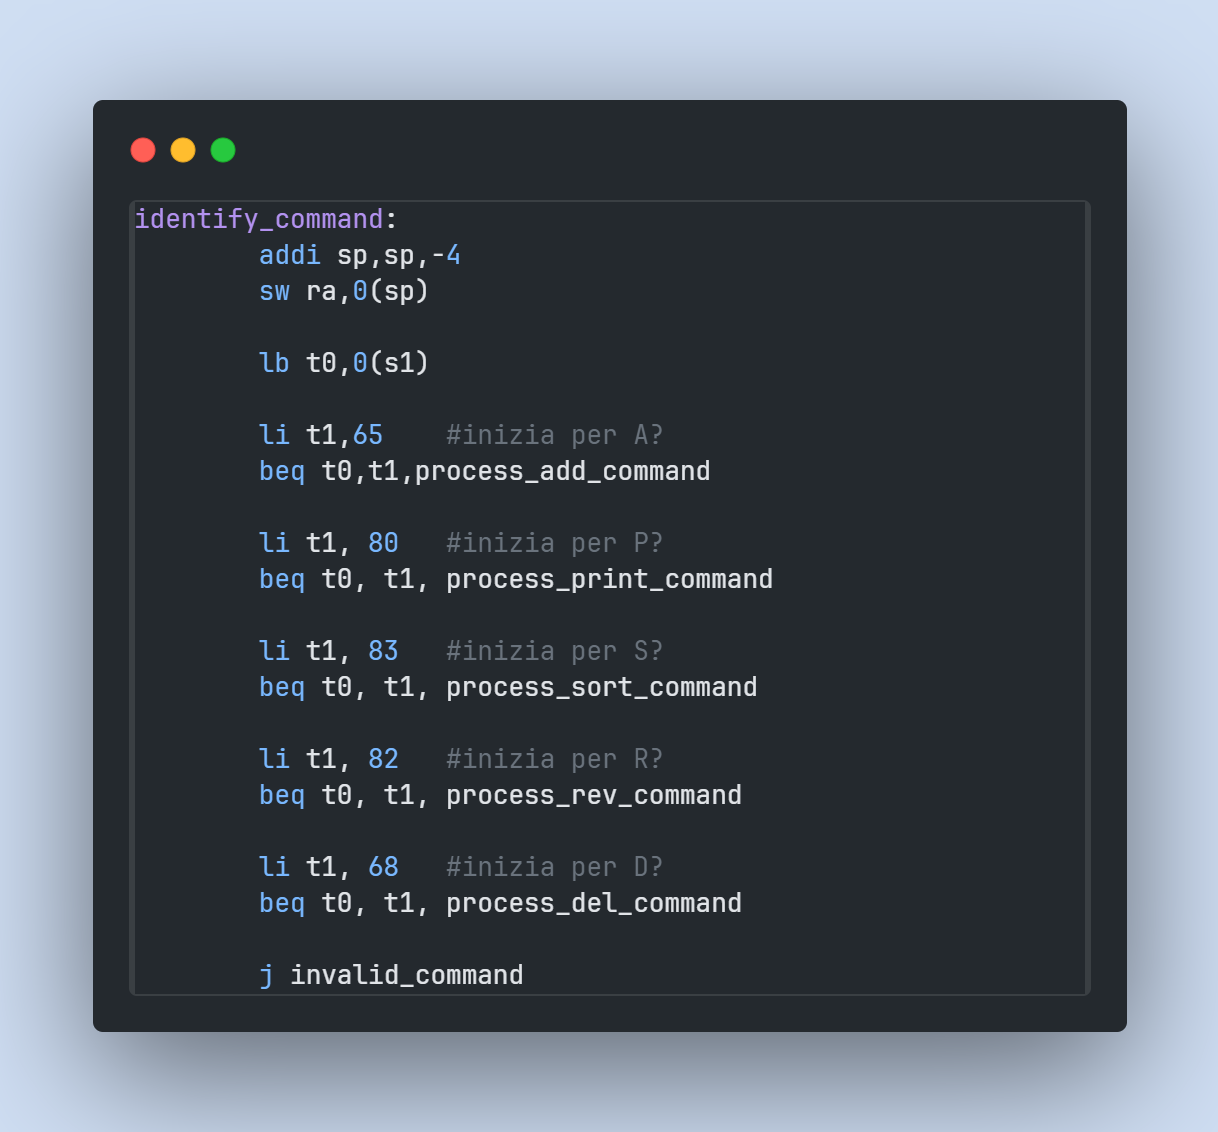
\includegraphics[width=0.40\linewidth]{img/identify_command.png}
                \label{fig1:1b}
            }
            \label{fig1}
            \caption[]{}
        \end{figure}
        
       Se il controllo non viene trasferito, scorro la stringa (tramite \textit{find\_next\_command}), finché non trovo una tilde o un fine stringa, per poi ritornare nel loop principale e ricominciare la fase di identificazione comando. \\
       Altrimenti,la procedura \textit{process\_\textbf{x}\_command} trasferisce il controllo a \textit{verify\_\textbf{x}\_format} (dove \textbf{x} è il comando in questione).
       Se il comando è correttamente formattato e finisce con un terminatore valido (spazio o $\sim$) allora la verifica termina correttamente (cioé il metodo ritorna \textbf{1} in  \textit{a1})\footnote[1]{\textit{Il valore di ritorno della funzione di validazione sarà in a1 per evitare interferenze con comandi che accettano parametri nel registro \textit{a0} come ADD e DEL}} e lo eseguo tramite \textit{jump-and-link} alla rispettiva procedura.\\ Terminata l'operazione avanzo di un carattere.

    \section{verify\_\textbf{x}\_format}
    
    \begin{mdframed}
        \texttt{parametri:} nessuno \\
         \texttt{ritorno:}\textit{a1}  (\textcolor{ForestGreen}{1 - successo}, \textcolor{Red}{0 - fallimento})\\
         \texttt{cosa fa:} ritorna se il formato del comando \textbf{x} è valido o meno

    \end{mdframed}
    La funzione di verfica controlla sequenzialmente
    \begin{enumerate}
        \item se i caratteri successivi sono quelli propri del comando in questione
        \item se il comando ha un parametro ammissibile (cioé un carattere ASCII fra 32 e 125
        \item se il comando ha un terminatore valido (tramite \textit{verify\_command\_terminator} che skippa eventuali spazi e controlla la presenza di un terminatore tilde/fine stringa valido 
        
    \end{enumerate}
    In caso di successo carica in \textit{a1} il valore 1 e ritorna con successo.\\
    In caso contrario vuol dire che è stata richiamata la procedura \textit{invalid\_format} che carica in \textit{a1} il valore 0 e ritorna al chiamante.
    \newpage
    \chapter{Funzioni}
    \justifying
    \section{Premessa}
    Le varie funzioni sono state implementate modularmente e sono state realizzate in modo da mantenere il più possibile valido il principio di regolarità, cruciale nell'architettura RISC-V. Tutte le funzioni che necessitano di parametri (cioé \textit{ADD} e \textit{DEL} li accettano nel registro \textit{a0}, mentre tutte le funzioni che devono restituire dei valori li restituiscono in \textit{a1}. Inoltre tutte le procedure salvano all'inizio

    \section{Funzioni principali}
    \subsection{ADD}
    \begin{mdframed}
        \texttt{parametri:} in \textit{a0} carattere ASCII (sarà il DATA del nodo) \\
         \texttt{ritorno:} nessuno \\
         \texttt{cosa fa:} aggiunge un carattere ASCII alla lista concatenata
    \end{mdframed}
    Per effettuare la ADD di un nodo, devo per prima cosa individuare un indirizzo di memoria di 5 byte libero, pertanto richiamo la procedura \textit{find\_next\_free\_addr} descritta di seguito, tra le procedure di supporto. Individuato l'indirizzo della prossima locazione di memoria libera, salva nel primo byte (deputato al DATA) il carattere passato come parametro e successivamente mi allineo ai successivi 4 byte, nei quali salverò l'indirizzo del prossimo nodo, che sarà nullo in quanto il nodo successivo non esiste.\\
    \uline{A questo punto distiguiamo il caso della prima ADD della catena dal caso di ADD successivo.}
    \begin{itemize}
        \item[$\diamond$]nel caso della prima ADD: aggiorno le variabili globali \textit{HEAD\_PTR} e \textit{LAST\_PTR} con l'indirizzo della testa del nodo appena inserito
        \item [$\diamond$]nel caso di nodo successivo: aggiorno il \textit{PAHEAD} del nodo precedente con l'indirizzo del nodo attuale e \textit{LAST\_PTR} con con l'indirizzo del nodo corrente.
    \end{itemize}
    \newpage
    \subsection{DEL}
    \begin{mdframed}
        \texttt{parametri:} in \textit{a0} carattere ASCII (occorrenze da eliminare) \\
         \texttt{ritorno:} nessuno \\
         \texttt{cosa fa:} elimina \textbf{tutti} i nodi contenenti quel carattere
    \end{mdframed}
    Se la lista non è vuota, inizia controllando la testa e se va eliminata, aggiorno HEAD\_PTR con il \textit{PAHEAD} di quel nodo (rendo quindi il nodo successivo la nuova testa). Dopo di che diminuisco il counter dei nodi e controllo nuovamente se il nodo diventato testa va anch'esso eliminato. Se la lista diventa vuota, aggiorno anche il \textit{LAST\_PTR} e termino.\\
    Altrimenti, se la testa non va eliminata, scorro tutti gli altri nodi e per ognuno, controlla il carattere del nodo a lui seguente e se coincide con il carattere da eliminare aggiorna di conseguenza i \textit{PAHEAD} del nodo precedente e del nodo successivo; quando arrivo all'ultimo nodo della catena, aggiorna il \textit{LAST\_PTR}.
    
    \begin{figure}[H]
            \centering
            \includesvg[width=0.75\linewidth]{img/after-del.svg}
            \caption{Esempio di funzionamento di DEL}
            \label{fig}
    \end{figure}


    \subsection{PRINT}
    \begin{mdframed}
        \texttt{parametri:} nessuno \\
         \texttt{ritorno:} nessuno \\
         \texttt{cosa fa:} stampa ordinatamente tutti i nodi della catena
    \end{mdframed}

    La stampa è gestita ricorsivamente, a partire dalla testa tramite la procedura \textit{print\_recursive} (che accetta in \textit{a0} un indirizzo, la quale stampa, se la HEAD non è zero (a causa di lista vuota o raggiungimento dell'ultimo elemento) il carattere di un nodo. Dopo di che, richiama ricorsivamente sé stessa, ma dopo aver aver scorso al nodo successivo e passando in \textit{a0} l'indirizzo del nodo successivo.\\
    Per quanto concerne la gestione della memoria, ad ogni ricorsione
    
    
    
    
\end{document}